\documentclass[onecolumn, 12pt]{article}
\usepackage[margin=0.75in]{geometry}
\usepackage{amsmath,amsthm,amsfonts,amssymb,amscd}
\usepackage{amsfonts}
% \usepackage{lastpage}
\usepackage{hyperref}
\usepackage{dirtytalk}
\usepackage{aas_macros}
\usepackage{natbib}
\usepackage{graphicx}

\hypersetup{
    colorlinks=true,
    linkcolor=blue,
    filecolor=magenta,      
    urlcolor=cyan,
}

\title{Detecting and dispositioning transiting exoplanets through phase-folded light curves}
\author{Michelle Chen}

\begin{document}

\maketitle

\section{Introduction}

Among the 2,600 transiting exoplanet candidates detected by NASA's Kepler space telescope during its nine-year-long mission, some were dismissed as False Positives (FPs) by an automated vetting procedure known as the Robovetter. Such a procedure is far from infallible. Numerous FP diagnoses can and have been overturned, resolving themselves as actual Planet Candidates (PCs) upon human inspection. A recent example would be the Earth-like Kepler-1649c: initially dispositioned by the Robovetter's Model-Shift Uniqueness test as an FP, it was determined by a team of transatlantic astronomers to be a PC. This was the focus of Vanderburg et al.'s 2020 publication, \say{A Habitable-zone Earth-sized Planet Rescued from False Positive Status.}

The following paper will focus on the habitability of exoplanet candidates, the automated process behind their (mis)identification, and the implications of this automation — how it should be balanced against human inspection.

\subsection{The habitability of exoplanets orbiting M-dwarf stars}

Many exoplanets — planets outside the Solar System that orbit around non-solar stars — possess atmospheric or surface-level conditions that would endear themselves toward inhabiting liquid water, and in turn, extraterrestrial forms of life. It is generally presumed within the field of astronomy that the mass of the star around which a planet orbits, as well as the composition of that planet's atmosphere, play a role in determining the pressure on the surface — and, in turn, the range of temperatures at which water would assume a liquid state (Vladilo et al. 2013). Stellar mass, for one, places limitations on the habitability of planetary systems, wherein both too high and too low of a mass may disqualify orbiting planets from habitability. At the upper bound, higher-mass stars typically experience shortened lifespans than lower-mass stars. Due to their higher rates of fuel consumption, resulting in a narrower window of time preceding stellar death, these high-mass stars generally do not allow benign conditions enough time to cultivate life before stellar death (Yang et al. 2013). Then, at the lower bound, very small stars — despite their longevities — tend to be faint. The redder wavelengths of their radiation translates to less temperate conditions within the atmosphere, not to mention the increased difficulty in detectability through both spectrographic and imaging procedures.

These questions of habitability — i.e. \textit{which stellar and planetary parameters are more hospitable than others?} — were foundational to the scientific objectives of NASA's 2009-2018 Kepler mission. In evaluating potentials for life outside earth, the Kepler space telescope hoped to determine the amounts of terrestrial-sized planets in habitable zones, as well as the characteristics of stars that harbored planetary systems, among other things. Although the mission endeavored at first to focus on Sun-like stars, its findings piqued interest in M-dwarf stars ($0.1M_{\bigodot} \lesssim M \lesssim 0.6M_{\bigodot}$), such as Kepler-1649 — the host to Kepler-1649c. Dressing $\&$ Charbonneau, in a 2015 publication, investigated the probabilities of terrestrial-sized planets' ($1.0-1.5 R_{\bigoplus}$) as well as \say{super-Earths'} ($1.5-2 R_{\bigoplus}$) existences around M-dwarfs. They concluded that, for orbital periods shorter than 200 days, and with planet radii of $1-4 R_{\bigoplus}$, there was a cumulative occurrence rate of $2.5 \pm 0.2$ planets per M-dwarf, therefore indicating a higher likelihood of habitability. Moreover, M-dwarfs are comparatively ubiquitous throughout the galaxy. They are the most common outcome of the star formation process within the Milky Way, such that two-thirds of all stars in the solar neighborhood (within 15 light-years from the Sun) are M-dwarf stars (Kroupa 2001). Contextualizing these factors with the longevity of M-dwarfs, as smaller stars that burn their fuel slower, has led numerous astronomers to believe that M-dwarfs may very well be the most promising stars for planetary hospitality (Vanderburg et al. 2020). This is the rationale of large numbers: because there are many of these stars, because these stars tend to host multiple planets, and because they tend to live for long periods of time, they open themselves up to life.

As an exoplanet orbiting around an M-dwarf star, then, Kepler-1649c becomes of interest. It is located 300 light-years from Earth, exhibiting a size only 1.06 times larger than its analog, and receiving roughly 75$\%$ the amount of starlight from its host star that Earth receives with the Sun. The aggregate of these factors increases the likelihood of liquid water on its presumably temperate surface. Granted, this was only determined after Vanderburg et al. \say{rescued} the object from its FP classification, and decided to further inspect the candidate's properties. It thus becomes pertinent to discuss why Kepler-1649c was dismissed in the first place, in spite of its now-known chances of habitability.

\subsection{The Robovetter's misclassification of Kepler-1649c}

The Kepler space telescope had produced a well-characterized planet candidate catalogue at the conclusion of its mission in measuring the frequency of Earth-sized planets in the galaxy. The catalogue was developed by downloading pixel time series from the telescope and processing them through the Kepler pipeline — which calibrated images, extracted light curves, and searched for periodic dimmings in the host star's flux. Using the transit method of planetary detection, these flux decrements are taken to represent the crossings of transiting/eclipsing planets between the light of sight to the host star; thus, they are aptly named Threshold Crossing Events (TCEs). They were then ran as input through the Robovetter's automated probabilistic screening procedure. To each TCE, the Robovetter assigned a \say{disposition score}: a measure of confidence in its classification of that TCE as a PC or FP. Scores near 0.0 indicate high-confidence FPs, whereas scores near 1.0 indicate high-confidence PCs. Kepler-1649c was scored a 0.374, and thus, was dispositioned as a not-transit-like FP.

To the False Positive Working Group (FPWG), formed by Vanderburg et al., this was unusual. The majority of TCEs dispositioned as FPs by the Robovetter possessed long orbital periods, ranging from 200 to as much as 500 days (Thompson et al. 2018). In contrast, Kepler-1649c's signal had a period $P \approx 19.535$ days. This was consistent with the dozens of its transits, undeviating in shape and depth over time, that the Kepler space telescope observed. In other words, there was little statistical foundation to indicate that Kepler-1649c was an FP. Therefore, the FPWG identified it as a possible PC, and investigated further.

Upon examining the strong quarterly variations in the photometric scatter of the Kepler pipeline's light curve, the FPWG hypothesized that the Kepler pipeline had applied suboptimal photometric apertures for certain quarters of time, such that minor pixelation errors would result in the \say{falling off} of certain TCEs from the aperture. This is what they suspected was the case with Kepler-1649c. Its host star had a high proper motion of $\mu$ = 168.2 milliarcseconds per year, which the pixel selection algorithm — assuming the star's position to be 2'' off from its true locale — failed to account for (Byrson et al. 2010). Moreover, Kepler-1649 is very faint, with a luminosity only $0.5\%$ that of the Sun. This further complicates the matter of optimizing photometric apertures to get them \say{just right.} As a result, Kepler-1649c had a significantly weaker transit signal in the pipeline photometry, and thus, appeared too low compared to the systematic noise level to be a PC.

\subsection{Reproducing phase-folded light curves for the Model-Shift Uniqueness test}

The FPWG improved upon the Kepler pipeline's selection of photometric apertures by extracting light curves from a set of 20 different apertures, and for each quarter, choosing the one that yielded the most photometrically precise curve. The new-and-improved light curve displayed a more consistent photometric scatter across quarters, as opposed to the large variations within the Kepler pipeline's — such that when the FPWG re-ran the Robovetter's Model-Shift Uniqueness test, Kepler-1649c passed as a viable PC. See Figure 1.

\begin{figure}[p]
\centering
\includegraphics[scale=0.5]{new light curve.png}
\caption{A phase-folded light curve produced by the FPWG. Kepler-1649b, a previously validated exoplanet orbiting the host star, is on the left; Kepler-1649c, the recently validated exoplanet joining the system, is on the right.}
\end{figure}

Using the reproduced Kepler light curve, the FPWG was able to fit 10 parameters for Kepler-1649c: the orbital period, radius ratio, semimajor axis, orbital inclination, transit impact parameter, transit duration, time of transit, planetary radius, flux, and temperature (in equilibrium), whose margins of error were derived via a Markov Chain Monte Carlo (MCMC) analysis of the curve. See Figure 2.

\begin{figure}[p]
\centering
\includegraphics[scale=0.9]{parameters.png}
\caption{The 10 parameters for Kepler-1649c. Uncertainties, or margins of error (represented by $\pm$), were found through an MCMC algorithm applied to the reproduced phase-folded light curve.}
\end{figure}

Due to the faintness of Kepler-1649, which prevents astronomers from simply making radial velocity observations, these stellar parameters are necessary in statistically validating Kepler-1649c's existence. The FPWG used \textit{vespa} software to calculate the relative likelihood that the transiting signal initially detected was truly due to a crossing planet, and not one of several possible FP scenarios, so as to further validate their findings from the reproduced light curve. They provided \textit{vespa} data on the candidate's orbital characteristics, transit light curve, as well as its host's stellar parameters, and found slightly ambiguous results. Due to Kepler-1649c's short transit duration, it was difficult for \textit{vespa} to distinguish its transit light curve from that of an extremely grazing eclipsing binary; this uncertainty materialized via a $\approx2\%$ calculated chance that the PC is actually an eclipsing binary. However, upon taking into account the previously verified Kepler-1649b within the same system, it would be astrophysically unviable for Kepler-1649c to be an eclipsing binary also orbiting the host star. In addition, real planets tend to be found in multi-transiting systems more often than FPs, which Kepler observed were more randomly sewn throughout the stars. With all considered, the FP probability for Kepler-1649c thus dwindles to the range of $1 \times 10^{-3} \sim 2 \times 10^{-3}$. This, alongside the careful reproduction of light curves for Kepler-1649c, suggests the importance of sprinkling in human investigation among the automated processing of large data sets.

\section{Reproducing phase-folded light curves via aperture photometry}

A noteworthy part of FPWG's production of light curves for Kepler-1649b and Kepler-1649c was aperture photometry: the selection of an aperture for each quarter that produced the most photometrically precise curve. This optimization was accompanied by their accounting for potentially diluting fluxes from nearby stars, referred to as \say{contaminants.}

The following original calculations will perform \textbf{Simple Aperture Photometry} on a variety of test cases to produce and compare light curves to those from Vanderburg et al.'s FPWG. To this end, it will use \textit{lightkurve}, a package for Kepler and TESS time series analyses, as well as \textit{matplotlib}, a data visualization library, to do so. Both run in Python 3.7. Because manual aperture optimization is beyond the scope of these calculations — rather, they will use the defaulted Kepler pipeline aperture — pixel optimization will be the focus instead. To recap: In investigating why Kepler-1649c failed the Robovetter's Model-Shift Uniqueness Test, the FPWG concluded that the fully automated pixel selection algorithm employed by the Kepler pipeline failed to account for the faintness of the host star, as well as its high proper motion. As a result, half-pixel errors resulted in Kepler-1649 remaining within the photometric aperture in some quarters, while falling outside of it entirely in others. This demonstrates the importance of pixel optimization, both through programmatic means and through human inspection.

\subsection{Carrying out Simple Aperture Photometry (SAP) via data-based programming on four cases of study}

The primary intention of the original calculations within this paper is to compare the FPWG's light curve of Kepler-1649c to representatives from the following categories: (1) A certified false positive (FP); (2) A confirmed planet whose host star exhibits *low* proper motion (ease of pixel optimization); (3) A confirmed planet whose host star exhibits *high* proper motion (difficulty in pixel optimization, much like Kepler-1649 itself); and, lastly, (4) an unclassified planet candidate (PC), so as to conclude with a non-automated dispositioning, modeling the work of Vanderburg et al.

For these comparisons, the paper will emulate aperture photometry via SAP. This begins with downloading all pixels from every quarter of the planet candidate's data set. Among those pixels, a select few are chosen programmatically, in a way that eliminates as much flux contamination as possible. These chosen pixels are then summed to a singular flux value, as well as for every image per time slice. The light curve is then cleaned up through a series of functions: \textit{flattening}, which removes long-term trends using a Savitzky-Golay digital filter; \textit{removing outliers}, which uses simple sigma clipping ($\sigma$-clipping; \textit{removing NaNS}, which takes out illegitimate infinite, or Not-a-Number (NaN), values; \textit{folding}, which folds the data at a particular time period of the x-axis; and \textit{binning}, which calculates the average flux in each statically incremented bin to reduce the overall time resolution of the plot. Note that all data will be extracted from the NASA Exoplanet Archive's cumulative Kepler Objects of Interest (KOI) database; additional stellar parameters will be taken from the SIMBAD astronomical database.

For Case 1's certified FP, KIC 892772 will be used as the representative. The TCE has a transit period of $5.09246539 \pm 4.39e-05$ days. Its initial light curve contains highly inconsistent amounts of photometric scatter with little to no transiting signs — as seen in Figure 3 — such that the initial dispositioning of FP goes unchallenged. Even after applying functions to optimize the light curve, there remains no transit signal to be found; see Figure 4. Yet, in spite of this, and KIC 892772's certified FP status, it would be procedurally sound to account for the possibility that the signal has been contaminated by a nearby star. Therefore, it is important to plot the target pixel files, to check for any interfering fluxes. Examining Figure 5, where the pre-selected region of pixels (masked as red) lies in the upper-left quadrant, it is notable that high flux from the central quadrant may indicate contamination. Therefore, by re-selecting the pixels to \say{mask} this central quadrant, one can investigate the source of interference; see Figure 6. This produces the light curve shown in Figure 7, characterized by a monotonically downward-sloping wave with low amplitude, and no transit signal in sight. The results from these light curves are thus in agreement with the dispositioning of KIC 892772 as an FP.

\begin{figure}[p]
\centering
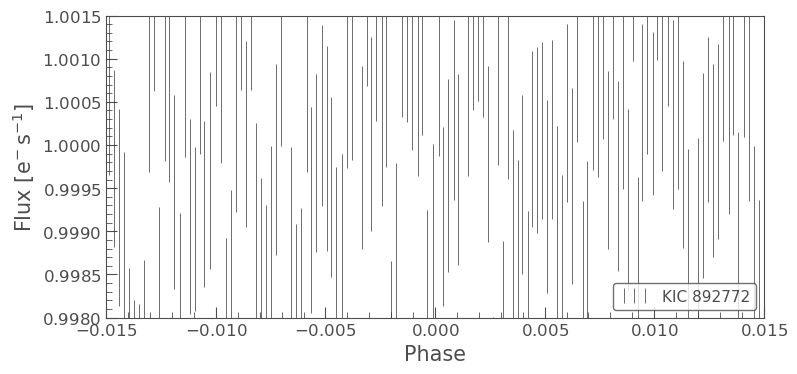
\includegraphics[scale=0.5]{892772-1.png}
\caption{\textbf{Case 1}: There is no transit signal in the light curve plotted for KIC 892772; this is in accordance with the subject's FP dispositioning.}
\end{figure}

\begin{figure}[p]
\centering
\includegraphics[scale=0.5]{892772_alt.png}
\caption{\textbf{Case 1}: Even optimizing the light curve with various folding, binning, etc. functions reveals no signs of a transit.}
\end{figure}

\begin{figure}[p]
\centering
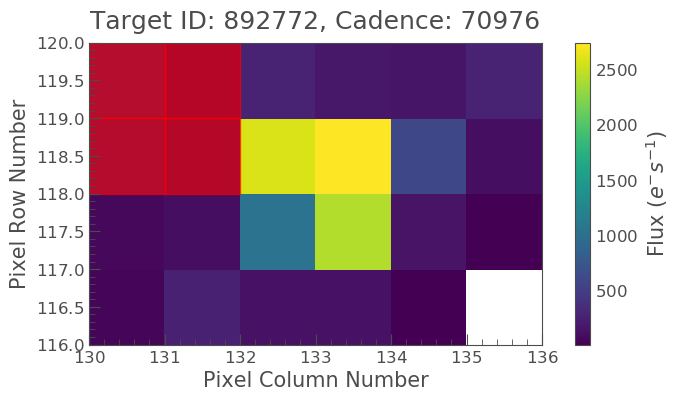
\includegraphics[scale=0.5]{892772-2.png}
\caption{\textbf{Case 1}: Plotting the target pixel files to check for interfering fluxes allows one to detect how high flux from the central, non-selected quadrant, may contain contamination worth investigating.}
\end{figure}

\begin{figure}[p]
\centering
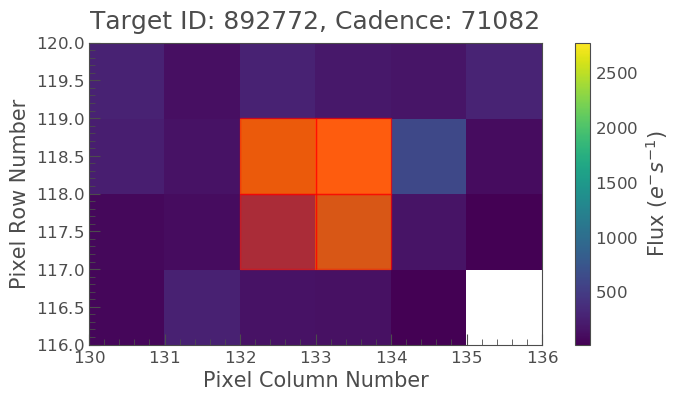
\includegraphics[scale=0.5]{892772-3.png}
\caption{\textbf{Case 1}: Masking the central quadrant, which previously showed signs of contamination.}
\end{figure}

\begin{figure}[p]
\centering
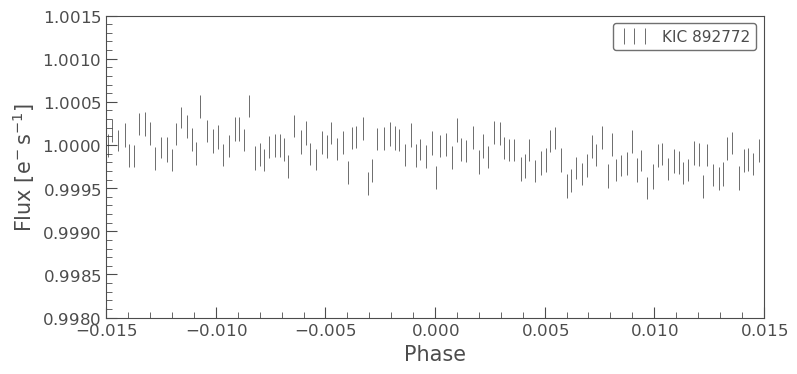
\includegraphics[scale=0.5]{892772-4.png}
\caption{\textbf{Case 1}: There are, again, no signs of a transit. Therefore, neither the contaminating flux nor the original signal disagree with the FP dispositioning.}
\end{figure}

Case 2's confirmed planet — specified to transit a host star with a low proper motion (PM) — can be represented by Kepler-227b (KIC 10797460). Confirmed as a planet in a 2014 publication by Rowe et al., the planet has an orbital period of $9.48803557 \pm 2.775e-05$ days. Its host star, Kepler-227, carries a low PM of $5.00003$ mas yr$^{-1}$; this was calculated through the Pythagorean theorem, provided $\mu_{\delta}=4.644 \text{ mas yr}^{-1}$ and $\mu_{\alpha *}=1.853 \text{ mas yr}^{-1}$. As a PC, Kepler-227b was dispositioned with a score of 1.0000, indicating high confidence in a PC classification. The production of a light curve for the subject agrees with this dispositioning: there are clear signs of a transit in Figure 8. Moreover, upon plotting the target pixel files, one finds that the reading is isolated (Figure 9). Because there is no risk of contamination outside the central quadrant that was selected, no re-selection is required.

\begin{figure}[p]
\centering
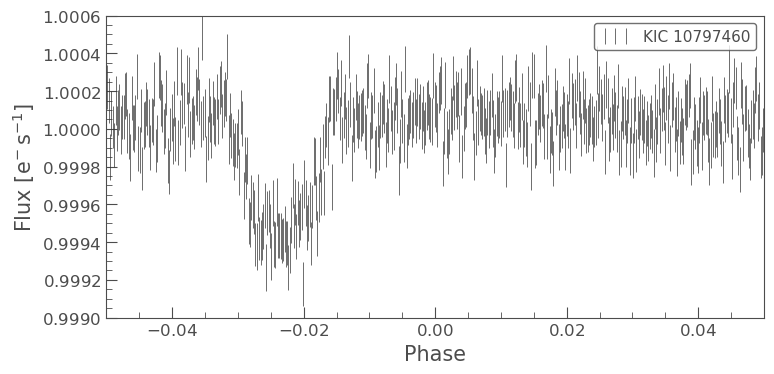
\includegraphics[scale=0.5]{10797460_updated.png}
\caption{\textbf{Case 2}: Producing a light curve for Kepler-227b reifies its classification as a true planet with the above transit signal.}
\end{figure}

\begin{figure}[p]
\centering
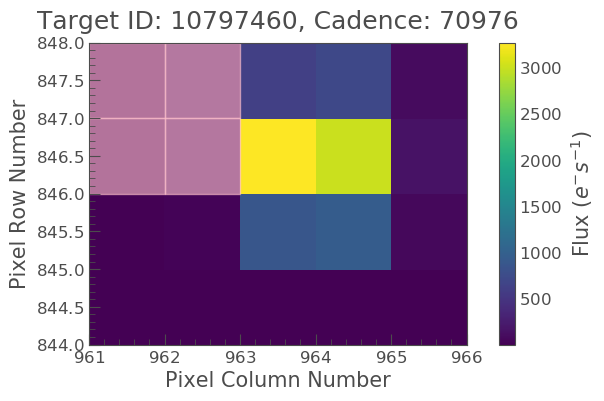
\includegraphics[scale=0.5]{10797460-2.png}
\caption{\textbf{Case 2}: By unmasking the selected central quadrant of pixels, one finds that there is no outside contamination.}
\end{figure}

Case 3's confirmed planet distinguishes itself from case 2's with a high PM; Kepler-42c (KIC 8561063) qualifies as a representative. It has a short orbital period of $0.453287416 \pm 1.02e-07$ days ($10.9$ hours), and its host star, located in the Cygnus constellation, carries a renownedly high PM of $\mu=427.682 \text {mas yr}^{-1}$ — which, again, was calculated via $\mu_{\alpha*}=93.126 \text {mas yr}^{-1}$ and $\mu_{\delta}=-417.420 \text { mas yr}^{-1}$. As a PC, Kepler-42c was initially assigned a disposition score of 0.0000, indicating high confidence in the automated FP classification, as well as further suggesting a direct correlation between high stellar PM and difficulties in aperture/pixel optimization. However, this classification was disproven in a 2012 publication by Muirhead et al.; the paper dispositioned all three transit signals detected around Kepler-42 as true planets: they came to be known as Kepler-42b, Kepler-42c, and Kepler-42d, respectively.

Due to low orbital period as well as high stellar PM, producing the light curve for Kepler-42c requires additional fine-tuning. Upon downloading pixel files from the fourth quarter, adjusting the x- and y-axes of the plot, and taking additional steps to flatten, fold, and remove outliers and infinite/NaN values, the plot in Figure 10 was produced. There is a clear transit signal at phase $\sim 0.325$. To be certain of no interfering fluxes, the target pixel files are also plotted — again, with the aperture mask in red — in Figure 11. Though there are dim fluxes adjacent to the mask, there is nothing bright enough so as to be capable of a misleading signal. Therefore, all plots agree with the original dispositioning of Kepler-42c as a bona fide planet.

\begin{figure}[p]
\centering
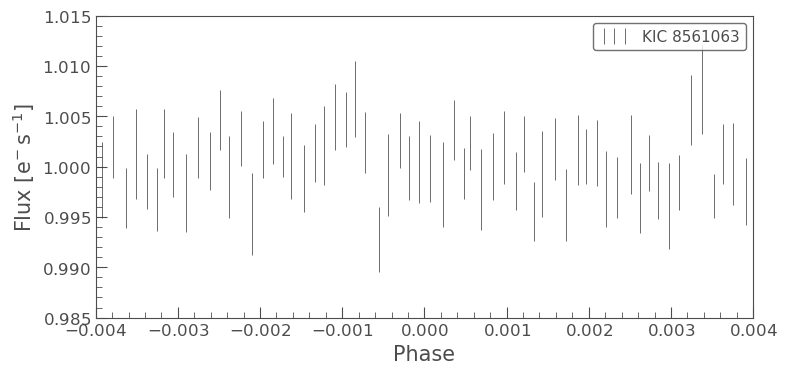
\includegraphics[scale=0.5]{8561063-1.png}
\caption{\textbf{Case 3}: The light curve for Kepler-42c, which, due to the high proper host star, required additional fine-tuning re: folding, binning, removing outliers, etc.}
\end{figure}

\begin{figure}[p]
\centering
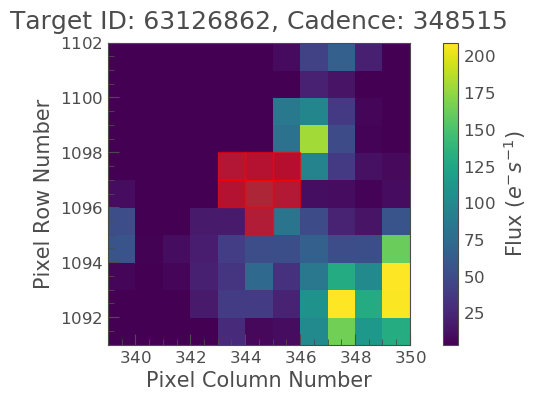
\includegraphics[scale=0.5]{8561063-2.png}
\caption{\textbf{Case 3}: Plotting the target pixel files (aperture mask in red) to check for contaminating nearby fluxes.}
\end{figure}

The final case, which focuses on manually dispositioning an unclassified PC, uses KIC 6679295 as its representative. The subject has a transit period of $24.5752524 \pm 0.0001782$ days, and its initial light curve demonstrates promising signs of a transit; see Figure 12. It becomes especially critical, for this unclassified subject, to decontaminate the light curve of any interfering fluxes. Upon plotting the target pixel files, seen in Figure 13, there emerges a nearby bright contaminant in the upper-leftmost quadrant, outside the central quadrant that has been masked. This is worth investigating, so one must re-mask to pursue this inquiry; the resulting plot of pixels is in Figure 14. Doing so allows one to then produce a light curve from the contaminant, which — as seen in Figure 15 — reveals no signs of a transit. Thus, it is clear that only KIC 6679295 has a planet signal. Therefore, it is with high confidence that one can disposition KIC 6679295 as a true planet, and not an FP.

\begin{figure}[p]
\centering
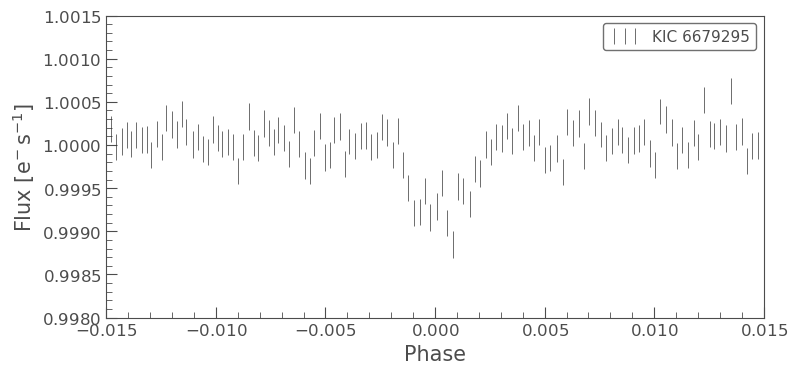
\includegraphics[scale=0.5]{6679295-4.png}
\caption{\textbf{Case 4}: The light curve produced for the unclassified KIC 6679295 shows clear signs of a transit.}
\end{figure}

\begin{figure}[p]
\centering
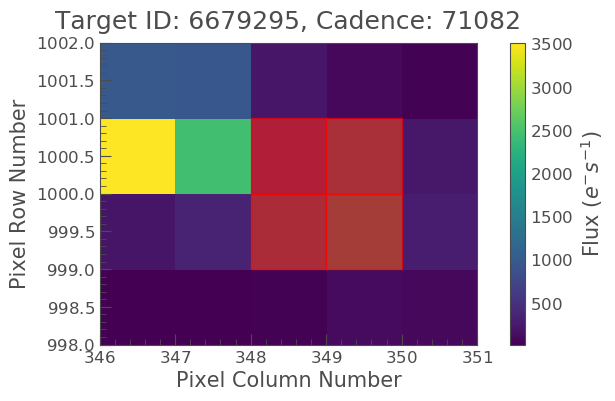
\includegraphics[scale=0.5]{6679295-1.png}
\caption{\textbf{Case 4}: Plotting the target pixel files for KIC 6679295 reveals possible contamination in the upper-left quadrant, outside the masked central quadrant (in red) of chosen pixels.}
\end{figure}

\begin{figure}[p]
\centering
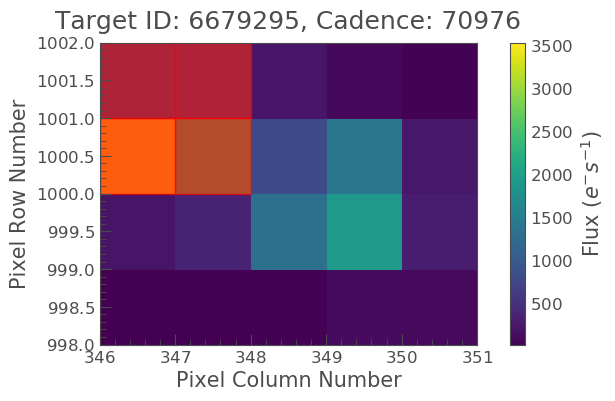
\includegraphics[scale=0.5]{6679295-3.png}
\caption{\textbf{Case 4}: Remasking to focus on the upper-left quadrant allows one to investigate signals from a potentially interfering flux.}
\end{figure}

\begin{figure}[t]
\centering
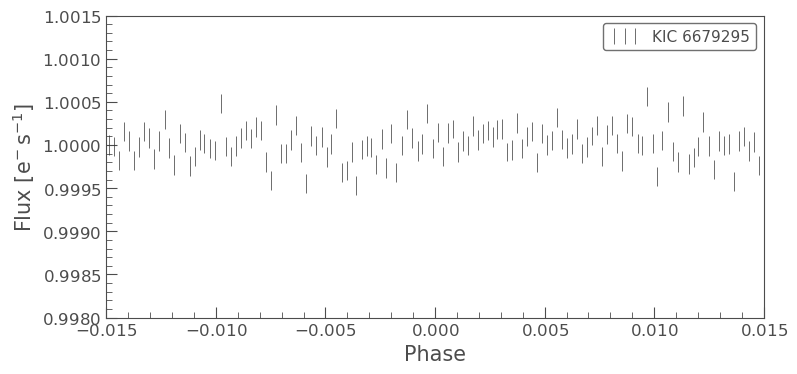
\includegraphics[scale=0.5]{6679295-2.png}
\caption{\textbf{Case 4}: After producing a light curve from the remasked pixels, it becomes clear that the flux does not come from a nearby transiting planet. KIC 6679295 should thus be dispositioned as a true planet.}
\end{figure}

\subsection{Analysis of calculations}

Aperture photometry does require some element of human inspection for optimal performance: in selecting apertures (in the case of the FPWG), or in selecting target pixels, as shown prior. Additionally, stellar parameters such as high proper motion and faintness weaken the detectability of transit signals around host stars. These should be taken into account when producing phase-folded light curves, for as seen with Kepler-42 in the third case — as well as Kepler-1649c — such factors necessitate additional optimization of the curve. Otherwise, photometric scatter will obscure the transit. This is what led originally to Kepler-1649c being dispositioned with a score of 0.0000, after all.

\section{Conclusions: Human inspection vs. automated vetting; A delicate balance}

Given the consistent increase in volumes of data, as well as the improvement of astronomical classification techniques, automated vetting processes are useful in the \say{triage} stage of sifting through bulk quantities of unidentified celestial objects. Tools such as the Robovetter, and its Model-Shift Uniqueness Test, have allowed NASA to produce an abundance of light curves and TCEs every month, significantly reducing the workload on individual astronomers. Efficiency, as well as statistical uniformity, are achieved at the cost of some individual disposition correctness, leading to incorrect vettings such as Kepler-1649c and Kepler-42c. Therefore, human inspection should be applied to strategically elected data samples from these sets. This would enable the field of astronomy to continually improve its algorithms so as to account for influential stellar parameters. By examining unique candidates from these samples, astronomers can learn more about the properties of exoplanets and their habitability, paving inroads for future discoveries.

\section*{References}

Bryson, S.T., Jenkins, J.M., Klaus, T.C., et al. \say{Selecting pixels for Kepler downlink.} \textit{Proc. SPIE.} 7740, 77401D, 2010.

\medskip

\noindent Dressing, C.D., \& Charbonneau, D. \say{The Occurrence Rate of Small Planets Around Small Stars.} \textit{ApJ.} 767 (95), 2013.

\medskip

\noindent Kroupa, P. \say{On the variation of the initial mass function.} \textit{ADS.} 322, 231. 2001.

\medskip

\noindent Muirhead, P.S., Johnson, J.A., Apps, K., et al. \say{Characterizing the Cool KOIs. III. KOI 961: A Small Star with Large Proper Motion and Three Small Planets.} \textit{ApJ.} 747 (2), 2012.

\medskip

\noindent Rowe, J.F., Bryson, S.T., Marcy, G.W., et al. \say{Validation of Kepler's Multiple Planet Candidates. III. Light Curve Analysis and Announcement of Hundreds of New Multi-planet Systems.} \textit{ApJ.} 784 (1), 2014.

\medskip

\noindent Thompson, S.E. et al. \say{Planetary Candidates Observed by \textit{Kepler}. VIII. A Fully Automated Catalog with Measured Completeness and Reliability Based on Data Release 25.} \textit{ApJ.} 2018.

\medskip

\noindent Vanderburg, A. et al. \say{A Habitable-zone Earth-sized Planet Rescued from False Positive Status.} \textit{ApJ.} 893 (1), 2020.

\medskip

\noindent Yang, J.; Cowan, N.B.; Abbot, D.S. \say{Stabilizing Cloud Feedback Dramatically Expands the Habitable Zone of Tidally Locked Planets.} \textit{ApJ.} 771 (2), 2013.

\end{document}
